
\documentclass{beamer}

\usepackage{algpseudocode}

\usetheme{Montpellier}
\usecolortheme{rose}

% page numbers, from
% https://tex.stackexchange.com/questions/137022/how-to-insert-page-number-in-beamer-navigation-symbols
\expandafter\def\expandafter\insertshorttitle\expandafter{%
  \insertshorttitle\hfill%
  \insertframenumber\,/\,\inserttotalframenumber}

\newcommand{\stanza}{ \\~\ }

\title{03. Heaps, Heapsort, and the Sorting Lower Bound}
\subtitle{CPSC 535 $\sim$ Spring 2019}
\author{Kevin A. Wortman}
\institute{ 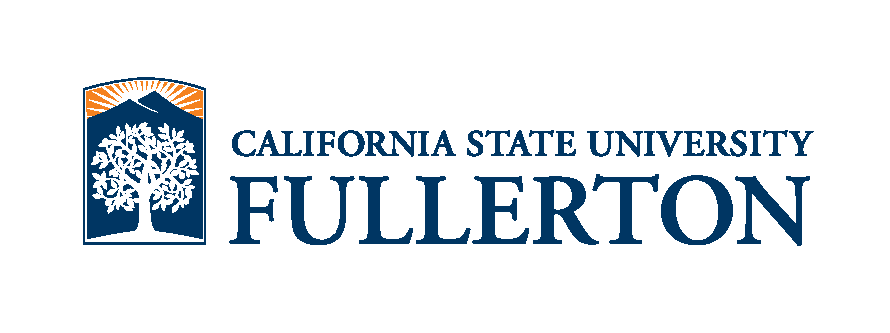
\includegraphics[height=2cm]{csuf-logo-cmyk} }
\date{February 11, 2019 \stanza

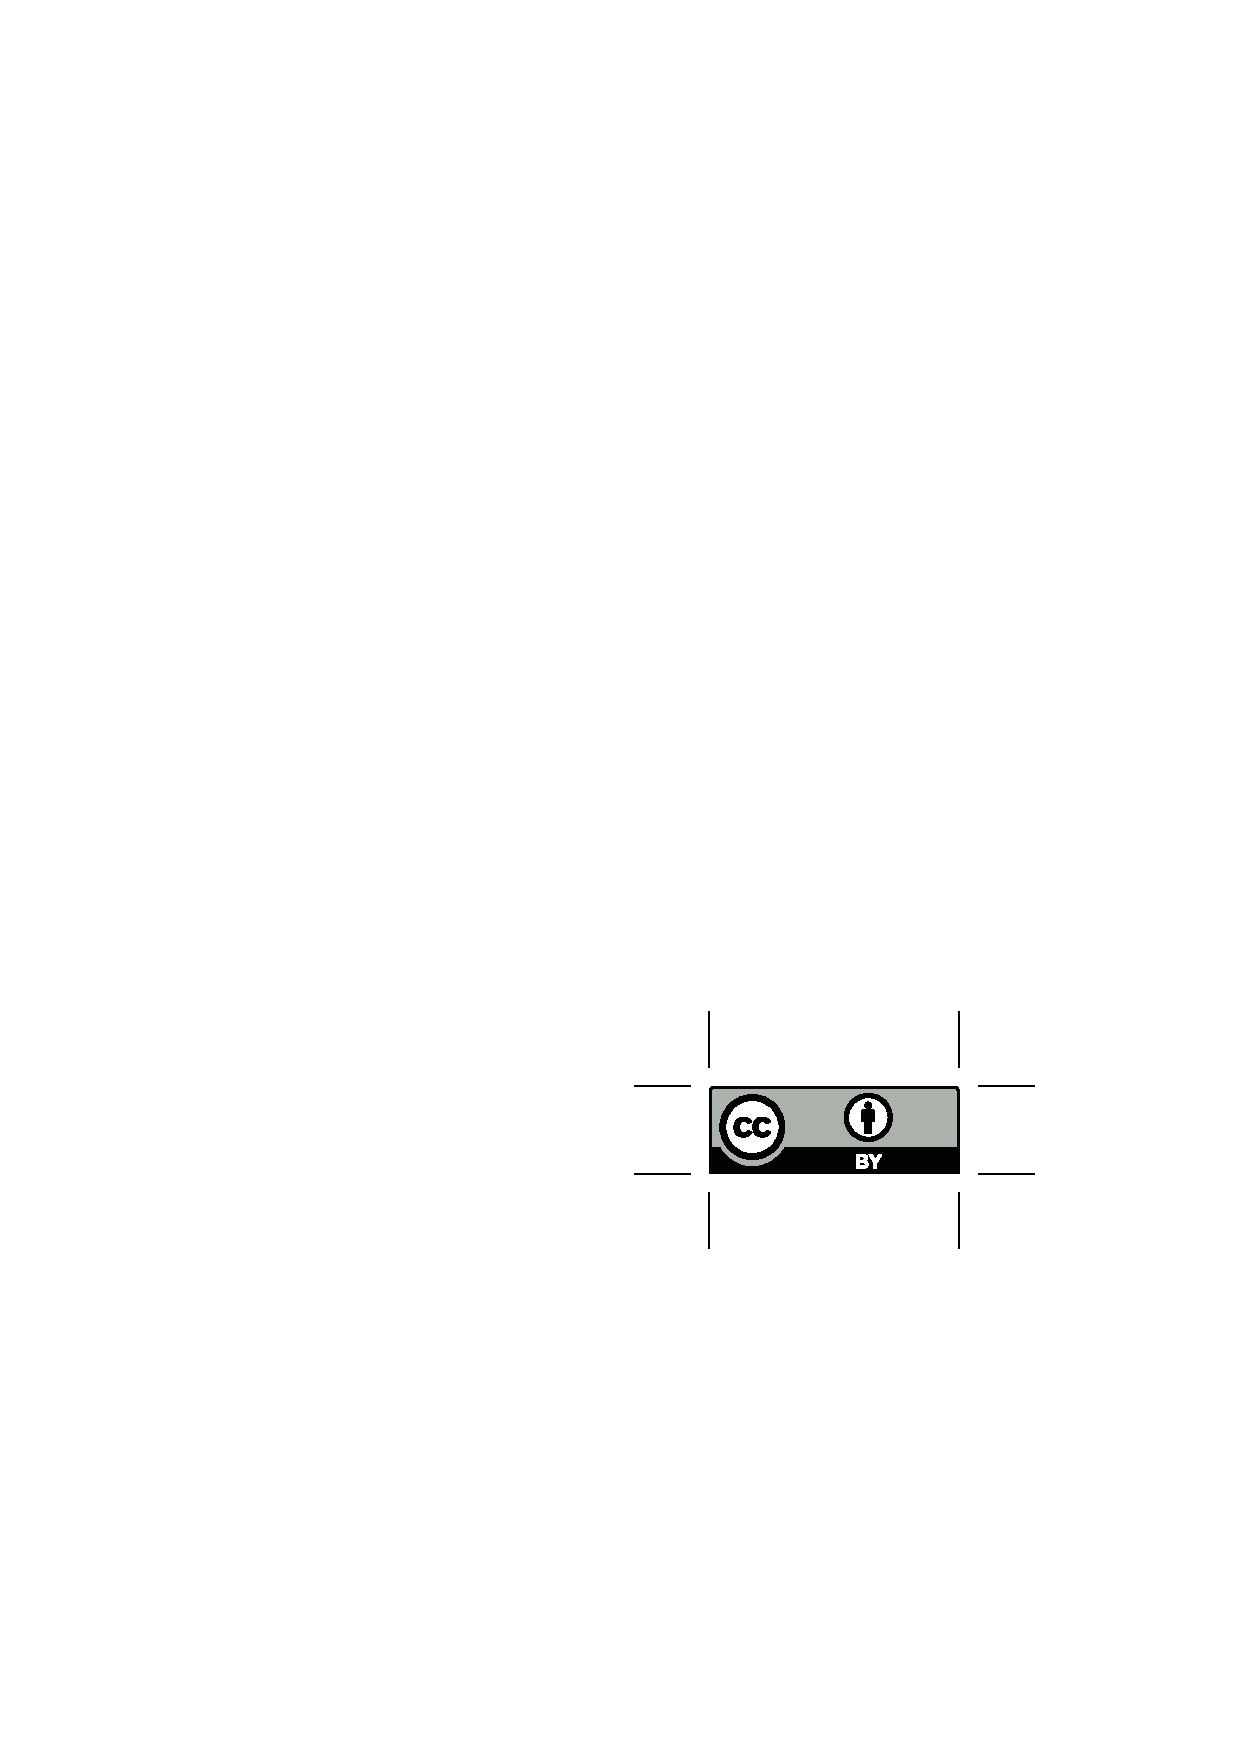
\includegraphics[height=14pt]{by} \\

{\tiny
This work is licensed under a
\href{http://creativecommons.org/licenses/by/4.0/}{Creative Commons Attribution 4.0 International License}.
}}

\begin{document}

\begin{frame}
  \titlepage
\end{frame}

\begin{frame} \frametitle{Heaps}

``Heap'' data structure in general
\begin{itemize}
  \item like binary search tree, but weaker order condition
  \item find min/max fast, usually $\Theta(1)$
  \item insert/delete-min/max fast, $\Theta(\log n)$ or even $\Theta(1)$
  \item search slow, $\Theta(n)$ \stanza
\end{itemize}

Applications
\begin{itemize}
  \item operating system scheduler
  \item accelerate algorithms: selection sort (heapsort),
    Prim's MST algorithm,
    Dijkstra's shortest paths algorithm, others
\end{itemize}
\end{frame}

\begin{frame} \frametitle{Big Picture}
\textbf{Big idea in computer science}: automata with simple local behavior can have amazing effects
when assembled at scale
\begin{itemize}
  \item finite states and Turing tape cells $\rightarrow$ Turing-complete computation
  \item CPU instructions $\rightarrow$ sophisticated software
  \item neural network nodes $\rightarrow$ teachable intelligent system
  \item hyptertext pages $\rightarrow$ the web
  \item compromised network hosts $\rightarrow$ distributed denial of service
  \item (today): tree nodes w/ different order and balance invariant $\rightarrow$ organize
    large datasets efficiently in different ways
\end{itemize}

\end{frame}

\begin{frame} \frametitle{Kinds of Heaps}

Like binary search trees and hash tables, there are many competing variations
of heap
\begin{itemize}
  \item binary heap (covered here)
  \item Fibonacci heap
  \item quake heap
  \item hollow heap \stanza
\end{itemize}

\emph{Heap memory} is a disparate concept and unfortunate naming clash

\end{frame}

\begin{frame} \frametitle{Binary Heap Order Invariant}

Let parent node $p$ have children $l, r$ \\
Recall \textbf{BST invariant}: $l.key < p.key < r.key$ \\
Binary \textbf{max-heap invariant}: $p.key \geq l.key$ and $p.key \geq r.key$ \\
(sketch) \stanza

Implies
\begin{enumerate}
  \item BST is totally sorted, but loosely balanced
  \item heap-order is ``half-baked'' sort; can tell parent comes before children,
    but siblings are unsorted relative to each other
  \item root must be overall maximum; that one element is perfectly sorted
  \item tradeoff: heap can be more tightly balanced than BST
\end{enumerate}

\end{frame}

\begin{frame} \frametitle{Max-Heap vs. Min-Heap}

\textbf{Max-heap}: \underline{maximum} key at root; $p.key \geq l.key, p.key \geq r.key$ \stanza

\textbf{Min-heap}: \underline{minimum} key at root; $p.key \leq l.key, p.key \leq r.key$ \stanza

No significant difference in implementation; swap $<$ for $>$ in \textbf{if} statements \stanza

Max-heap is more convenient for sorting in non-decreasing order, so we'll focus on that \stanza

(Min-heap is more convenient for non-increasing sort, Prim, Dijkstra)

\end{frame}

\begin{frame} \frametitle{Binary Heap Balance Invariant}

\textbf{Height} of a node: distance from bottom (root is highest) \stanza

\textbf{Depth} of a node: distance from root (leaves are deepest) \stanza

Heap is nearly-perfectly-balanced
\begin{itemize}
  \item every level except the bottom is completely full
  \item bottom level: full on the left side, may be missing elements on the
    right side (sketch)
  \item (N.B. insisting on a completely perfect tree is impractical because it requires $(n+1)$ is a power of 2)
  \item $\implies$ tree height $\Theta(\log n)$
\end{itemize}

\end{frame}

\begin{frame} \frametitle{Arrayed Binary Heap}

\emph{Arrayed} structure: packs something into an array
\begin{itemize}
  \item locality of reference $\implies$ good cache performance
  \item only one allocate/free per structure lifetime $\implies$ fast constant factors
\end{itemize}

Arrayed max-heap:
\begin{itemize}
  \item partially-filled array $A[1, \ldots, n]$ stores $k$ heap elements in $A[1, \ldots, k]$ for $k \leq n$
  \item root/maximum always in $A[1]$
  \item $PARENT(i) = \lfloor i/2 \rfloor$
  \item $LEFT(i) = 2i$
  \item $RIGHT(i) = 2i+1$
  \item $PARENT, LEFT, RIGHT$ are $\Theta(1)$ and ordinarily only 1-2 CPU instructions each
\end{itemize}
\end{frame}

\begin{frame} \frametitle{Create Heap Operation}
  \begin{algorithmic}[1]
    \Function{CREATE-MAX-HEAP}{A}
    \Require $A$ is an array of size $n$ that may become a heap
    \Ensure $A$ is a valid, empty, heap
    \State $A.heapsize = 0$
    \EndFunction
  \end{algorithmic}

  (Trivial pseudocode, but still worthwhile to write this down so that each operation
   is encapsulated and crystal clear.)

  Clearly $\Theta(1)$ time
\end{frame}

\begin{frame} \frametitle{Find-Max Operation}
\begin{algorithmic}[1]
  \Function{MAX-HEAP-MAXIMUM}{A}
  \Require $A$ is a valid, non-empty heap
  \Ensure returns the maximum key in $A$
  \State \Return $A[1]$
  \EndFunction
\end{algorithmic}

Again, straightforward and clearly $\Theta(1)$ time
\end{frame}

\begin{frame} \frametitle{Max-Heapify Intro.}

$MAX-HEAPIFY(A, i)$
\begin{itemize}
  \item assuming $LEFT(i)$ and $RIGHT(i)$ obey the order invariant, ensure $i$
    obeys the invariant
  \item $A[i]$ might be OK, or might need to ``float down'' deeper
  \item Delete-max and build are easy once we have $MAX-HEAPIFY$
  \item $\Theta(\log n)$ time
\end{itemize}
\end{frame}

\begin{frame} \frametitle{Max-Heapify Pseudocode}
{\small
\begin{algorithmic}[1]
  \Function{MAX-HEAPIFY}{A, i}
  \Require $A$ is a heap, $A[LEFT(i)]$ and $A[RIGHT(i)]$ are heap-ordered
  \Ensure $A[i]$ is heap-ordered
  \State $l = LEFT(i), r = RIGHT(i)$
  \If{ $l \leq k$ and $A[l] > A[i]$}
    \State largest = $l$
  \Else
    \State largest = $i$
  \EndIf
  \If{ $r \leq k$ and $A[r] > A[largest]$}
    \State largest = $r$
  \EndIf
  \If{ largest $\ne i$ }
    \State $swap(A[i], A[largest])$
    \State $MAX-HEAPIFY(A, largest)$
  \EndIf
  \EndFunction
\end{algorithmic}
} % small
\end{frame}

\begin{frame} \frametitle{Max-Heapify Analysis}
\begin{itemize}
  \item Suppose the subtree rooted at $i$ contains $n$ elements
  \item Everything except recursion takes $\Theta(1)$ time
  \item One recursive call on one child
  \item Worst-case: the child subtree we recurse into has more elements
  \item Balance invariant $\implies$ at least 1/3 elements on right side $\implies$ at at most $2/3$ elements in worst case
  \item $T(n) = T(\frac{2}{3}n) + \Theta(1)$
  \item $T(n) \in \Theta(\log n)$ by master theorem case 2
  \item \textbf{Pushing the envelope}: for any fraction $f<1$,
    including $f>\frac{1}{2}$,
    $T(fn)+\Theta(1) \in O(\log n)$
\end{itemize}
\end{frame}

\begin{frame} \frametitle{Delete-Max Operation}

Idea: grab rightmost node on bottom level, move it to root, heapify root (sketch)

\begin{algorithmic}[1]
  \Function{MAX-HEAP-DELETE-MAX}{A}
  \Require $A$ is a valid non-empty heap
  \Ensure the maximum key in $A$ is removed and then returned
  \State $max = A[1]$
  \State $A[1] = A[A.heapsize]$
  \State $A.heapsize = A.heapsize - 1$
  \State $MAX-HEAPIFY(A, 1)$
  \State \Return $max$
  \EndFunction
\end{algorithmic}

Analysis: $\Theta(1)$ plus $MAX-HEAPIFY$ so $\Theta(\log n)$
\end{frame}


\begin{frame} \frametitle{Increase Key Operation}
$A[i]$ ``floats up'' until it is either in heap-order, or becomes the root \stanza

\begin{algorithmic}[1]
  \Function{MAX-HEAP-INCREASE-KEY}{A, i, key}
  \Require $A$ is a valid heap, $1 \leq i \leq n, key > A[i]$
  \State $A[i] = key$
  \While{ $i>1$ and $A[PARENT(i)] < A[i]$}
    \State $swap(A[i], A[PARENT(i)])$
    \State $i = PARENT(i)$
  \EndWhile
  \EndFunction
\end{algorithmic}

$\Theta(\text{depth of } A[i]) = \Theta(\log n)$ time

\end{frame}

\begin{frame} \frametitle{Insert}
\begin{algorithmic}[1]
  \Function{MAX-HEAP-INSERT}{A, key}
  \Require $A$ is a valid heap, $A.heapsize < n$
  \State $A.heapsize = A.heapsize + 1$
  \State $A[A.heapsize] = - \infty$
  \State $MAX-HEAP-INCREASE-KEY(A, A.heapsize, key)$
  \EndFunction
\end{algorithmic}

Analysis: $\Theta(1)$ plus $MAX-HEAP-INCREASE-KEY$, so $\Theta(\log n)$
\end{frame}

\begin{frame} \frametitle{Build-Heap}
\textbf{Online/incremental construction}: build structure one element at a time \stanza

\textbf{Offline construction/build}: given $n$ elements all at once, build valid data structure \stanza

Offline is often faster, by constant factors or even asymptotically \stanza

Leaves are trivially in heap order and live in $A[\lfloor n/2 \rfloor+1, \ldots, n]$ \stanza

Parents might be out of heap-order and live in $A[1, \ldots, \lfloor n/2 \rfloor]$ \stanza

Just heapify all the parents! \stanza
\end{frame}

\begin{frame} \frametitle{Build-Heap Pseudocode}
  \begin{algorithmic}[1]
    \Function{BUILD-MAX-HEAP}{A}
    \Require $A[1, \ldots, n]$ may or may not be in heap-order
    \Ensure $A[1, \ldots, n]$ is in heap-order
    \State $A.heapsize = n$
    \For {$i$ from $\lfloor n/2 \rfloor$ down to 1}
      \State $MAX-HEAPIFY(A, i)$
    \EndFor
    \EndFunction
  \end{algorithmic}
\end{frame}

\begin{frame} \frametitle{Build-Heap Analysis}
Loose analysis: if $A[i]$ is at height $h$, $MAX-HEAPIFY$ takes $\Theta(h)$;
  $h \in O(\log n)$, so each call is $O(\log n)$; $n$ calls; so $O(n \log n)$ \stanza
(Correct but loose upper bound.)

Fact about balanced binary trees:
\begin{itemize}
  \item Sum of all node \textbf{depths} is $\Theta(n \log n)$
  \item Sum of all node \textbf{heights} is $\Theta(n)$
  \item Observe that 1/2 of ndoes are at height 0, 1/4 at height 1, 1/8 at height 2, etc.
  \item (sketch)
\end{itemize}

$n$ calls to $MAX-HEAPIFY$ take time $\Theta(\sum_i (\text{ height of } i)) = \Theta(n)$ \\
$\therefore$ $BUILD-MAX-HEAP$ takes $\Theta(n)$ time
\end{frame}

\begin{frame} \frametitle{Arrayed Binary Max-Heap Summary}

\begin{center}
  \begin{tabular}{lc}
    \textbf{Operation} & \textbf{Time Compl.} \\
    Create empty heap & $\Theta(1)$ \\
    Find maximum element & $\Theta(1)$ \\
    Insert one element & $\Theta(\log n)$ \\
    Delete and return maximum element & $\Theta(\log n)$ \\
    Increase key of previously-inserted element & $\Theta(\log n)$ \\
    Build $n$-element heap offline & $\Theta(n)$ \\
  \end{tabular}
\end{center}

\end{frame}

\begin{frame} \frametitle{Heapsort Intro}
\begin{itemize}
  \item Reduction to max-heap operations
  \item Selection sort: find maximum unsorted element, place at back of sorted array, repeat until done
  \item Use max-heap to accelerate "find maximum" step
  \item Convenient: if heap holds $k \leq n$ elements, it occupies
    $A[1, \ldots, k]$
  \item Remaining $n-k$ elements $A[k+1, \ldots, n]$ are free to hold sorted elements
\end{itemize}

High-level heapsort
\begin{enumerate}
  \item Build-heap; all $n$ elements hold a valid heap
  \item Delete-max; removes maximum element from heap zone, vacates one element in array
  \item Move the old max into the vacancy
  \item Repeat until done
\end{enumerate}
\end{frame}

\begin{frame} \frametitle{Heapsort Pseudocode}
  \begin{algorithmic}[1]
    \Function{HEAPSORT}{A[1, \ldots, n]}
    \Ensure $A$ is in non-decreasing order
    \State $BUILD-MAX-HEAP(A)$
    \For {$i$ from $n$ down to 2}
      \State $A[i] = MAX-HEAP-DELETE-MAX(A)$
    \EndFor
    \EndFunction
  \end{algorithmic}
(Observe: no need for $i=1$ iteration.) \stanza

Analysis
\begin{itemize}
  \item build-heap $= \Theta(n)$
  \item $(n-1)$ iterations of loop $\times \, \Theta(\log n)$ each
  \item $= \Theta(n \log n)$ total
\end{itemize}
\end{frame}

\begin{frame} \frametitle{Sorting Lower Bound}
So far all our sorts have compared elements to each other, e.g. $A[i] < A[j]$ \\
(insertion, selection, merge, heap sort; also quick sort) \stanza

Q: what is the minimum number of comparisons adequate to sort? \stanza

A: enough to decide which of the $n!$ permutations of $A$ would be in order \stanza

Binary search through a set of $N$ things takes $\lceil \log_2 N \rceil$ steps \\
$\implies $ correct sort makes $\geq \lceil \log_2 n! \rceil$ comparison operations \\
$= \Omega(n \log n)$ comparisons

$\therefore$ every comparison-based sorting algorithm takes $\Omega(n \log n)$ time \\
(\textbf{sorting lower bound})
\end{frame}

\begin{frame} \frametitle{Optimal Algorithms}
\textbf{Optimal Algorithm}: time complexity matches problem's lower bound \stanza

E.g.
\begin{itemize}
  \item Proven $\Omega(n \log n)$ lower bound for sorting
  \item Merge sort, heap sort take $\Theta(n \log n)$ time
  \item $\implies$ merge sort, heap sort are \textbf{optimal}
\end{itemize}

(Heap sort is theoretically superior because it is in-place.
Practical constant factors depends on whether allocation (mergesort) or cache misses (heapsort) are costlier.)
\stanza

Optimal algorithms are the end-goal of algorithm design and lower-bound analysis.
\end{frame}

\begin{frame} \frametitle{Epilogue --- Sorted Order vs. Heap Order}
We can sort by building a heap/BST and then retrieving elements in order. \stanza

Sorting lower bound $\implies$ that process \textbf{must} be $\Omega(n \log n)$

\begin{center}
\begin{tabular}{lll}
\textbf{Phase of sorting} & \textbf{BST} & \textbf{heap} \\
Build structure & $\Theta(n \log n)$ & $\Theta(n)$ \\
Retrieve in order & $\Theta(n)$ & $\Theta(n \log n)$ \\
\end{tabular}
\end{center}
Whack-a-mole: a $\Omega(n \log n)$ phase inevitably pops up somewhere! \stanza

Heap-order is not organized enough to be asymptotically significant, which is
 why it can be $o(n \log n),$ and maintain a stronger balance invariant than
 BSTs.

\end{frame}

\end{document}
